% -----------------------------------------------
% Vlastní text práce (kapitoly práce)
% -----------------------------------------------

% -----------------------------------------------
\chapter{Semiconductor detectors with p-n junction}
% -----------------------------------------------
Semiconductor structures have unique properties that make them useful for more than just particle/photon detection. There are many types of semiconductor detectors, starting with conventional photoresistors and photodiodes for light intensity measurements with a spectral range from infrared to UV. For low intensities and single photon events there are avalanche photodiodes (APDs). When the whole image needs to be captured, matrix detectors such as CCD and CMOS cameras can be used. In nuclear and particle physics, semiconductor detectors for X-rays, gamma rays and other particles are becoming increasingly common. For more complex measurements, such as particle trajectories, matrix drift or strip detectors may be the right choice. For gamma spectroscopy, p-n junction detectors are essential. To detect Mössbauer 14.4 keV gammas our primary choice are the Si PIN diodes for direct detection due to the high detection efficiency under 25 keV \cite{SiCdTe}. 
%The semiconductor structures has unique properties, which make them usable not only for a particle/photon detection. There are many types of semiconductor detectors starting with the conventional photoresistors and photodiodes for light intensity measurements with spectral range from infrared to UV. For low intensities and single photon events there are avalanche photodiodes (APDs). If there is a need for capturing the entire image, the matrix detectors can be employed, such as the CCD and CMOS cameras. On the field of nuclear and particle physics, the semiconductor detectors of x-ray, gamma and other particles are becoming more and more common. For more complex measurements such as the particles' trajectories the matrix drift or strip detectors can be the right choice. The essential role for gamma spectroscopy have the p-n junction detectors.


\section{The structure of semiconductor}
Individual atoms are characterised by the well-known discrete energy levels, but in the case of solid crystals there is another model to describe the energy levels - the band structure. In this model, the energy levels are so close to each other that they almost form a continuum. This difference in behaviour is due to a periodic potential within the crystal lattice. However, the electron energy $E_{\textrm{c}}$ is not the only quantum number that describes the behaviour of electrons within the periodic potential. By solving the Schrödinger equation using the so-called Bloch theorem, we conclude that the second important quantum number is the wave vector $\vec{k}$. These two quantum numbers are bounded by the dispersion relation $E_{\textrm{c}} = E_{\textrm{c}}(\vec{k})$, which is characteristic of each crystal and may play a role in the transition of electrons between bands.
%The single atoms are characterized by the well-known discrete energy levels, but in the case of solid crystals, there is another  model describing the energy levels - the band structure. In this model the energy levels are very close each other that they nearly form a continuum. This different behaviour is a result of a periodical potential inside the crystal lattice. However, the electron energy $E_{n}$ is not the only quantum number describing the behaviour of electrons inside the periodical potential. By solving Schrödinger equation with the help of so-called Bloch's theorem, we come to a conclusion that the second important quantum number is the wave vector $\vec{k}$. These two quantum numbers are bounded together by dispersion relations $E = E(\vec{k})$, which is characteristic for every crystal and may play role when it comes to transitions of electrons between bands.



\subsection{Direct and indirect semiconductors}
The shape of the dispersion relations $E_{\textrm{c}}(\vec{k})$ divides the semiconductors into two categories - direct and indirect semiconductors. For direct semiconductors the energy minimum in the conduction band and the energy maximum in the valence band have the same $\vec{k}$, so the transition can occur after the $E_{\textrm{g}}$ is supplied. In the case of indirect, the minimum and maximum have different $\vec{k}$. To make the transition, additional momentum must be supplied (e.g. by phonons) or the energy supplied must be much greater to allow the transition to the higher state with the same $\vec{k}$.  
 
 
 
%The shape of dispersion relations $E(\vec{k})$ divides the semiconductors into two categories - direct and indirect semiconductors. For direct semiconductors the energy minimum in conduction band and the energy maximum in valence band have the same $\vec{k}$, so the transition can occur after the $E_{\textrm{g}}$ is supplied. In case of indirect the minimum and maximum have different $\vec{k}$. To make transition, additional momentum has to be server (for example by phonons) or the supplied energy must be much larger to allow transition to the higher state. %with the same $\vec{k}$.  
%The Si crystal is an indirect semiconductor.


\subsection{Band structure}
The basic difference between conductors, insulators and semiconductors is the valence and conduction band structure. In conductors, the valence band overlaps the conduction band. The electrons in the conduction band can move almost freely throughout the crystal. For insulators, there is no overlap and the energy gap $E_{\textrm{g}}$ between the two bands is so large that it makes any electron transitions almost impossible. However, in the case of semiconductors, the $E_{\textrm{g}}$ is small enough to allow the electron to jump into the conduction band and leave the hole in the valence band after receiving enough energy - in the form of thermal energy $E_{\textrm{T}} = kT$, electric field $E_{\textrm{s}} = -e\phi$ or photon $E_{\textrm{photon}} = \hbar \omega_{\textrm{photon}}$. The last one is the most important because it allows us to use semiconductors as detectors. Both the electron and the hole take part in the conduction.
%The basic difference between conductors, insulators and semiconductors is the valence and conduction band structure. In case of conductors, the valence band overlaps the conduction band. The electrons in conduction band can move nearly freely throughout the crystal. For insulators, there is no overlap, and the energy band gap $E_{\textrm{g}}$ between the two bands is so high, that it makes any transitions of electrons nearly impossible. However, in the case of  semiconductors, the $E_{\textrm{g}}$ is small enough to allow the electron to jump into the conduction band leaving the hole in valence band after receiving a sufficient amount of energy - in form of thermal energy $E_{\textrm{T}} = kT$, electric field $E_{\textrm{s}} = -e\phi$ or photon $E_{\textrm{photon}} = \hbar \omega$. The last one is the most important, because it allows us to use the semiconductors as detectors. Both the electron and hole participates on conduction.


\subsection{Occupation of states}
The occupation probability of states in the band structure is given by the Fermi-Dirac distribution, since the electrons are the fermions with the exclusion rules. The possible occupied state where the occupation probability falls below 50 $\%$ is called the Fermi level with Fermi energy $E_{\textrm{F}}$. 
For an ideal pure semiconductor at $T=0$ K the $E_{\textrm{F}}$ is in the centre of the band gap. With increasing temperature the Fermi level in most materials moves upwards towards the conduction band.
%The occupation probability of states in band structure is given by Fermi-Dirac distribution since the electrons are the Fermions with the exclusion rules. The possible occupied state where occupation probability drops below 50 $\%$ is called the Fermi level with Fermi energy $E_{\textrm{F}}$. 
%For ideal pure semiconductor at $T=0$ K, the $E_{\textrm{F}}$ lies in the middle of the band gap. With increasing temperature, in most materials the Fermi-level moves upper towards the conduction band.

\subsection{Semiconductor Crystals}
Semiconductor materials are usually in the form of a crystal with a diamond structure (two FCC lattices bonded together), where the lattice atoms are bonded together by a covalent bond. However, in real crystals there are also defects and impurities that can change the functionality. The impurities can be intentionally added to enhance the desired properties in a process called doping. 
\par
There are several suitable materials for the construction of ionising radiation detectors. Among them the well-known is Ge, which has very good energy resolution but requires cooling. Another suitable material is Si. Si photodiodes have a high detection efficiency below 25 keV and are easy to manufacture, since many other semiconductor devices are made of Si. In the case of wide-spectrum X-ray and gamma-ray detectors, CdTe can provide sufficient parameters. The manufacture of semiconductors for detection purposes involves many complicated processes because the detector requirements for crystal purity are very high.
%The semiconductor materials have usually form of a crystal of diamond structure (two FCC lattices bounded together.) with the lattice atoms bounded by a covalent bond. However in real crystals there are also defects and impurities which may alter the functionality. The impurities can be added on purpose to enhance the properties we seek in procedure called doping. 
%\par
%There exist several suitable materials for the construction of ionizing radiation detectors. Among them the well-known is Ge, which has very good energy resolution, but on the other hand requires cooling. Another suitable material is Si. Si photodiodes have a great detection efficiency under 25 keV and they are easily fabricated since many other semiconductor devices are being made of Si. In case of wide-spectre x-ray and gamma ray detectors the CdTe can provide the sufficient parameters. The fabrication of semiconductors for purposes of detection includes many complicated processes, because the detector requirements on crystal purity are very high.




 
\section{The p–n junction}
Intrinsic semiconductors have a limited range of applications. We can alter the behaviour by adding specific impurities and create an extrinsic semiconductor. The Si atom has 4 valence electrons which form a covalent bond with other Si atoms. If the Si atom is replaced by an atom with 5 valence electrons, one of them will have a very weak bond.
By doping the intrinsic semiconductor with these atoms we create the $n$-type with additional electrons localised almost in the conduction band. However, the crystal as a whole remains neutral. Similarly, doping with atoms with only 3 valence electrons will create holes in the valence band - the $p$-type.
These atoms create energy levels in the band structure, but at room temperature they are all mostly ionised and participate in conduction. The full theoretical treatment of doping is very complex, taking into account many other quantum and statistical physics aspects, and is not useful for the purposes of this thesis. 

\par
The special effects arise when $p$-type and and $n$-type are bound together. The holes of the $p$ type and the electrons of the $n$ type will start to diffuse into the other region. However, this movement alters the charge density, leading to the creation of a built-in voltage, which in the end cancels out the diffusion. This creates the depleted region, where there are no free carriers. 
\par
Another theoretical view is that the electrons will rearrange because the Fermi level must be the same throughout the crystal, whereas for the stand-alone $p$ type the Fermi level is closer to the valence band and for the $n$ type closer to the conduction band. The potential created in this way equalises the different Fermi levels.
%The intrinsic semiconductors have only a little field of applications. We can alter the behaviour by adding a specific impurities and create an extrinsic semiconductor. The Si atom has 4 valence electron which form a covalent bond with other Si atoms. If Si atom is replaced with atom with 5 valence electrons, one of them will have a very weak bond.
%By doping the intrinsic semiconductor with these atoms we create the $n$-type with additional electrons, which are nearly localized in conduction band. However, the crystal as whole stays neutral. Similar way doping by atoms with only 3 valence electrons, there will be holes in valence band - the $p$-type.
%In band structure these atoms create energy levels in band structure, but in room temperatures, they are all mostly ionized and participate on conduction. The full theoretical treatment of doping is very complex, considers many other quantum and statistical physics aspects, and have no use for the purposes of this thesis. 
%
%\par
%The special effects will arise when $p$-type and and $n$-type are bound together. The holes from $p$-type and electrons from $n$-type will start to diffuse to the other region. However, this movement alter the charge density, which leads to creation of built-in voltage which in the end cancels the diffusion. This creates the depleted region, where are no free charge carriers. 
%\par
%Another theoretical view is that the electrons will rearrange, because the Fermi-level has to be same throughout the crystal, while the Fermi-level for stand-alone $p$-type is nearer to the valence band and for $n$-type is nearer to the conduction band. The potential created this way equalizes the different Fermi levels. 

\par
The p-n junction can be connected to the supply voltage ( known as a bias) in two ways. The first possibility is the forward connection - the $p$ layer to plus and $n$ to minus. Increasing the voltage in this type of connection causes the size of the depleted layer to decrease until it disappears completely (bias voltage is opposite to the built-in voltage). The absence of the depleted layer makes the p-n junction conductive. The second possibility is the reverse - $p$ to minus and $n$ to plus. Increasing the voltage also increases the size of the depletion layer (bias goes with the built-in voltage). Since the size of the depletion layer is crucial for detection, semiconductor detectors are operated in reverse connection.


\par
The p-n junction has many unique properties that are commonly used in the form of classical diodes. However, it is also crucial for detection because the free carriers (if produced at all) in the depleted layer are pushed towards the electrodes by the electric field and form a photocurrent.

\par
For design purposes in electronic circuits, detectors are usually modelled as classical p-n diodes connected to the bias source in the reverse direction. In the case of detection, the detector can also be modelled as a current source.


\par
The p-n junction has its characteristic capacitance, which depends on the size of the depleted layer and therefore on the bias voltage.
This capacitance plays an important role as it affects the dynamic parameters of the detection circuits and modifies the overall frequency spectra.
%The p-n junction can be connected to supply voltage (refereed as bias) in two ways. First possibility is the connection in the forward direction - the $p$ layer on plus and $n$ on minus. Increasing the voltage in this type of connection causes the reduction of the size of the depleted layer with  the until it completely vanishes (bias voltage goes against built-in voltage). The lack of the depleted layer makes the p-n junction conductive. Second possibility is the reverse direction - $p$ on minus and $n$ on plus. Increasing the voltage increases the size of depletion layer as well (bias goes with built-in voltage). Since the size of depletion layer is crucial for detection, the semiconductor detectors are operated in reverse direction.
%
%
%\par
%The p-n junction has many unique properties, which are commonly used in form of classical diodes. However, it is also crucial for the detection since the free charge carriers (if somehow created) in depleted layer are pushed towards electrodes by electric field and form a photocurrent.
%
%\par
%For the purposes of design in electronic circuits, the detectors are usually modelled as classical p-n diodes, which are connected to the source of the bias voltage in reverse direction. In case of detection, the detector can be also modelled as a current source.
%
%
%\par
%The p-n junction has its characteristic capacitance, which depends on the size of the depleted layer, and thus also on the bias voltage.
%This capacitance plays a significant role since it affects the dynamical parameters of the detection circuits and alters the entire frequency spectra.

%There is also one more problem with the diffusion of electron and holes which has to be considered. It is the diffusion of charge carriers from the $p$ and $n$ layers to the metal ohmic contacts on electrodes, which can form an unwanted electric field and a potential barrier across the contact. To prevent this from happening, the regions around the ohmic contacts are highly doped to reduce the potential barrier size. 


\section{Detection mechanism}
The detection of a particle or photon is based on its interaction with the detector material - in semiconductors the formation of electron-hole pairs is observed. This can be achieved by the interaction mechanisms described in previous chapters, which differ for each type of particle and energy. In the case of low energy gamma, the two main mechanisms involved in the production of charge carriers are the photoeffect (internal) and Compton scattering.

\par
The main purpose of the semiconductor as a detector is to perform a linear conversion of the particle/photon energy into the free charge carriers - electrons in the conduction band and holes in the valence band. The average energy required to create a single electron-hole pair is usually a fixed constant - in Si it is $\epsilon = 3.6$ eV \cite{Lutz_2007}. Since Si is an indirect semiconductor, this value is not equal to the gap energy, which is lower ($E_{\textrm{g}} = 1.12$ eV).  

\par
The gamma photon hitting the detector first interacts with a single electron. When the photoeffect takes its place, the primary electron with an energy much higher than the thermal excitation will ionise electrons from all over the valence band, pushing them into higher states from the conduction band. These conduction band electrons de-excited to lower conduction band states and the holes redistributed to the upper valence band states. This de-excitation process releases energy and leads to a cascade of further excitations and interactions, producing many electron-hole pairs - the charge cloud. The number of generated electron-hole pairs $n$ is simply given by the relation:
%The detection of a particle or a photon is based on interaction with the detector material - in semiconductor the creation of electron-hole pairs is observed. This could be achieved by interaction mechanisms described in previous chapters, which differ for every type of particle and energy. In case of low-energy gamma the two main mechanisms, which take place in producing the charge carriers, are photo-effect (internal) and Compton scattering.
%
%\par
%The main purpose of semiconductor as a detector, is to perform a linear conversion of the particle/photon energy into the free charge carriers - electrons in conduction band and holes in valence band. The average energy needed to create a single electron-hole pair is usually a fix constant - in Si it is $\epsilon = 3.6$ eV \cite{Lutz_2007}. Since the Si is an indirect semiconductor, this value is not equal to gap energy, which is lower ($E_{\textrm{g}} = 1.12$ eV).  
%
%\par
%The gamma photon striking the detector firstly interacts with a single electron. If the photo-effect takes its place, the primary electron with energy much higher than the thermal excitation will ionize the electrons from all over the valence band pushing them into higher states from conduction band. These Electrons in conduction band de-excite themselves into lower states of conduction band and the holes redistribute themselves to the upper states in valence band. This de-excitation process releases energy again and that leads to the cascade of further excitations and interactions, which produce many electron-hole pairs - the charge cloud. Number of generated electron-hole pairs $n$ is simply given by relation:


\begin{equation}
n = \frac{E_{\textrm{gamma}}}{\epsilon}.
\end{equation}

\par
Compton scattering results in energy distortion and gamma spectrum degradation. Compton without any other subsequent interaction (Compton again or photoeffect) is typical for thin detectors because there is not sufficient thickness to stop the scattered photon again.

\par
An ideal very thick detector could solve this problem, because all possible interactions and all subsequent sub-interactions would take place inside the detector, resulting in electron-hole generation. Such a detector would have only the full energy peaks without any other unwanted counts. However, the construction of such a detector is very complicated due to the many technical and manufacturing problems that arise with increasing dimensions. 

\par
In a p-n junction, the charge carriers generated in the depleted layer are pushed towards the electrodes by an internal electric field. The electronics accumulate the charge and convert it into a voltage pulse signal, which is then analysed to extract the energy information. Since the depleted layer is the only part where detection can occur, it is obvious that it should be as large as possible for detector purposes. 
\par
To achieve the larger dimensions of the detection part, the p-n junction can be upgraded to a p-i-n junction, which contains an additional intrinsic layer between the $p$ and $n$ parts, acting as a fixed size depleted layer. The detectors with p-i-n junction are called PIN photodiodes. The additional intrinsic layer reduces the capacitance but increases the time it takes for charge carriers to leave the detector.
%The Compton scattering results into the energy distortion and gamma spectrum devaluation. The Compton without any other following interaction (Compton again or photoeffect) is typical for thin detectors since there is insufficient thickness to stop the scattered photon again.
%
%\par
%An ideal very thick detector could solve this problem, because every possible interaction and all the following sub-interactions will happen inside the detector and will result into electron-hole generation. The detector of this kind would have only the full energy peaks without any other unwanted counts. However, construction of such detector is very complicated due to the many technical and manufacturing problems arising with increasing dimensions. 
%
%\par
%In case of p-n junction the created charge carriers in depleted layer are pushed towards electrodes by internal electric field. The  electronics accumulates the charge and converts it into the voltage pulse signal, which is then analysed to extract the energy information. Since the depleted layer is the only part where the detection can occur, its obvious that for detector purposes it should be large as possible. 
%\par
%To achieve the greater dimensions of the detection part, the p-n junction can be upgraded to p-i-n junction, which contain additional intrinsic layer between $p$ and $n$ part, which work as fix size depleted layer. The detectors with p-i-n junction are referred as PIN diodes. The additional intrinsic layer decreases the capacitance, but increases the time needed for charge carriers to exit the detection part.

\section{Main noise sources and resolution limitations}
Detection efficiency and energy resolution are strongly affected by noise that alters the signal. While some negative effects are caused by outside conditions such as temperature or by noise in the electronics, some originate strictly from the properties of the semiconductor material and can only be minimised during the preparation of the crystal.
%The detection efficiency and the energy resolution are strongly dependent on noise which alters the signal. While some negative effects are caused by outer conditions such as temperature or by noise in electronics, some originate strictly from semiconductor material properties and only chance to minimize them is during the crystal's preparation.

\subsection{Fano noise}
The physical effect within the semiconductor itself that limits the measured energy resolution is the fact that not all of the particle's energy is converted into charge carriers. A fraction of the energy can be consumed to induce lattice vibrations (phonons). Statistically, the relative resolution can be described by the following equation:
%The physical effect inside the semiconductor itself which limits the measured energy resolution is the fact that not all of the particle's energy is transformed into charge carriers. Some fraction of energy can be consumed to induce lattice vibrations (phonons). Statistically the relative resolution can be described by following equation:
\begin{equation}
\frac{\Delta E}{E} = 2.35\sqrt{\frac{F\epsilon}{E}},
\end{equation}
where $E$ is the energy of the incoming particle, $\epsilon$ is the average energy required to produce a single pair, and $F$ is a Fano factor. The Fano factor is a special statistical constant that describes the dispersion in the counting process. If we consider the case of 14.4 keV gamma in Si ($\epsilon = 3.6$ eV, $F = 0.12$), the $\frac{\Delta E}{E}$ is equal to 1.3 $\%$ and $\Delta E$ is 185.4 eV. This resolution is sometimes called intrinsic, because the real resolution is much worse.
%where $E$ is incoming particle's energy, $\epsilon$ is the average energy needed for the single pair creation and $F$ is a Fano Factor. Fano Factor is a special statistical constant which describes the dispersion in counting process. If we consider the case of 14.4 keV gamma inside Si ($\epsilon = 3.6$ eV, $F = 0.12$), the $\frac{\Delta E}{E}$ is equal to 1.3 $\%$ and $\Delta E$ is 185.4 eV. This resolution is sometimes called intrinsic, because the real resolution is much worse.




\subsection{Thermal noise}
It has been mentioned that the electrons can also be excited by thermal fluctuations. However, since many of the detector materials are indirect semiconductors, the thermal excitations are carried by the intermediate states within the band gap. These states originate from imperfections and impurities in the crystal lattice. The electrons and holes originating from this effect can join the charge cloud generated by the detected particle and reduce the SNR. This phenomenon is commonly referred to as dark current. Dark current is also increased by an applied bias.
\par
Thermal fluctuations are much more significant for materials that require less energy to excite the electrons to the conduction band, such as Ge. These detectors must always be operated at low temperatures. Even room temperature can lead to the breakdown and destruction of a detector. For Si, the valence and conduction bands are further from each other, so thermal fluctuations are not as critical.
%It was mentioned that the electrons can be also excited by thermal fluctuations. However, since the many of detector's materials are indirect semiconductors, the thermal excitations are carried through the intermediate states inside the band gap. These states have the origin in imperfections and impurities inside the crystal lattice. The electrons and holes originating from this effect can join the charge cloud generated by detected particle and decrease the SNR. This phenomenon is usually called dark current. The dark current is also increased by applied bias voltage.
%\par
%The thermal fluctuations are much more significant for materials which require less energy to excite the electrons to the conduction band such as Ge. These detectors always have to be operated at low temperatures. Even the room temperature can lead up to the breakdown and destruction of a detector. For Si, the valence and conduction band are more distant, so the thermal fluctuations are not so critical.


\subsection{Recombination and trapping}
The effect that counteracts successful carrier collection, and thus affects detection efficiency and energy resolution, is recombination. In pure crystals, the electron can only recombine with a hole if they have the same $\vec{k}$. However, in real crystals there are impurities that allow carriers to recombine - recombination centres. The charge collection must take much less time than the carriers need to recombine. 
\par
Another effect caused by the same impurities is trapping. The trapping centres capture the electron or hole and release it after a certain time. This effect alters the signal pulses and can reduce the maximum possible counting rate.
\par
Energy levels near the centre of the band gap are primarily responsible for recombination and trapping, which means that the impurities causing this are not the impurities added by doping, as these have their extra energy levels near the bands. 
%The effect which goes against the successful collection of charge carriers and thus affects the detection efficiency and the energy resolution is recombination. In pure crystals, the electron can recombine with hole only when they have the same $\vec{k}$. However, inside real crystals, there exist impurities, which allow carriers to recombine - recombination centres. The charge collection must take much less time than it takes the carriers to recombine. 
%\par
%Another effect caused by the very same impurities is trapping. The trapping centres capture electron or hole and release it after certain time. This effect alter the signal pulses and can decrease maximum possible counting rate.
%\par
%Energy levels near the centre of band gap are primary responsible for recombination and trapping, which means that the impurities causing this are not the impurities which were added in doping, because these have their additional energy levels near the bands. 


\section{Structure and parameters of Si PIN detector}
One of the most important parameters is the size of the photosensitive area, which must be as large as possible for effective radiation collection. This area must be treated with extreme care, as any damage, adsorption of impurities or condensation due to high ambient humidity will reduce the active photosensitive area.
\par
For detection purposes, the dimensions of all three layers (P, I and N) of the p-i-n semiconductor structure must be carefully designed. 
Obviously, the most important layer dimensions for the interactions within the detector are those parallel to the direction of incident radiation - the thicknesses of both the P and I regions.
The dead region (P) must be as thin as possible to reduce the probability that the particle will interact at a location where the generated charge cloud would recombine almost immediately. The active depleted layer (I) must be thick enough to allow all interactions to take place within itself. The schematic of a PIN photodiode can be seen in the figure \ref{SiPIN}.
%One of the most important parameter is the size of the photosensitive area, which has to be as large as possible for effective collection of radiation. This area has to be treated with extreme caution since every damage, adsorption of impurities or dew condensation due to the high environmental humidity reduces the active photosensitive area.
%
%\par
%For detection purposes, the dimensions of all three layers (P,I and N) of the the p-i-n semiconductor structure have to be laid out carefully. 
%It is obvious that for the interactions inside the detector the most crucial layer dimensions are those, which are parallel to the direction of incident radiation - the thicknesses of P and I regions.
%The dead region (P) has to be thin as possible to reduce probability that the particle interacts in place where the generated charge cloud would nearly immediately recombine. The active depleted (I) layer has to be thick enough to make all the interactions happen inside itself. The schematic of PIN photodiode can be seen in the figure \ref{SiPIN}.


\begin{figure}[H]
 \centering
 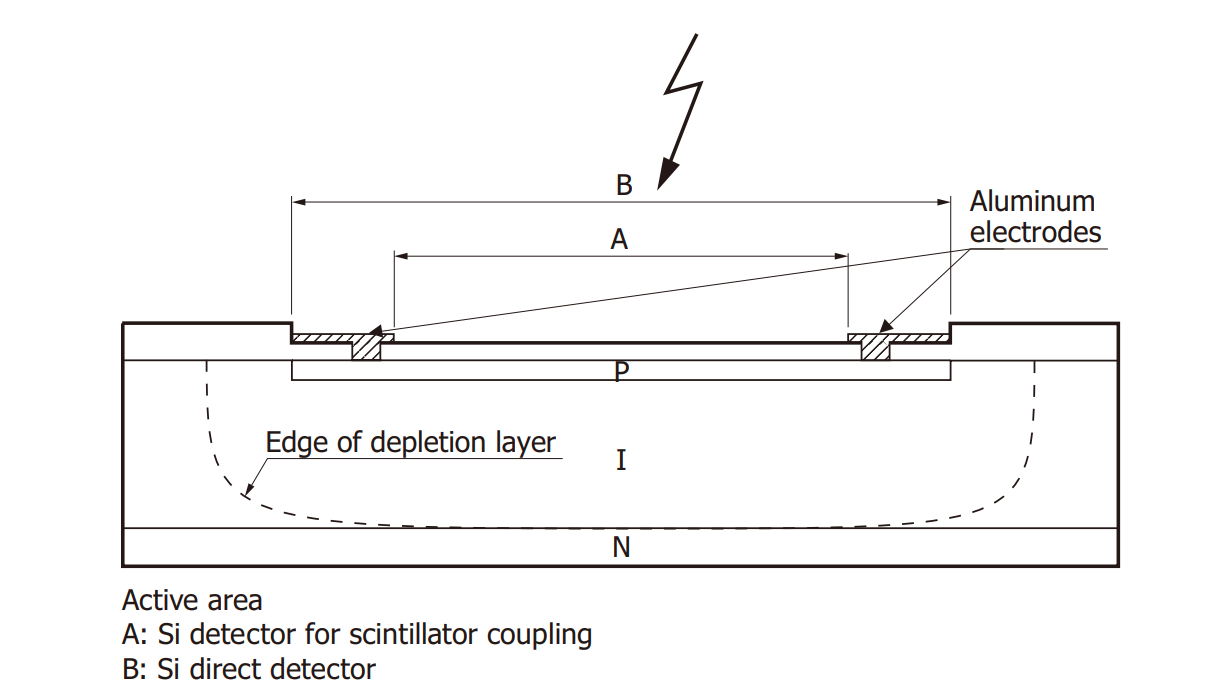
\includegraphics[scale=0.35, angle = 0]{./pictures/SiPINScheme.png}
 \caption{Cross section of Si detector for scintillator coupling and Si direct detector \cite{SiPINdirect}.}
 \label{SiPIN}
 
\end{figure}



\section{Available Si PIN detectors}
For testing, we chose a professional Hamamatsu S14605 PIN diode and two commercial PIN diodes: BPW34 - visible and near infrared radiation detector, OPF430 - originally designed for use in optical communications.
%For testing we have chosen one professional Hamamatsu S14605 PIN diode and two commercial PIN diodes: BPW34 - visible and near infrared radiation detector, OPF430 - originally designed to be used in optical communications.  

\begin{figure}[H]
 \centering
 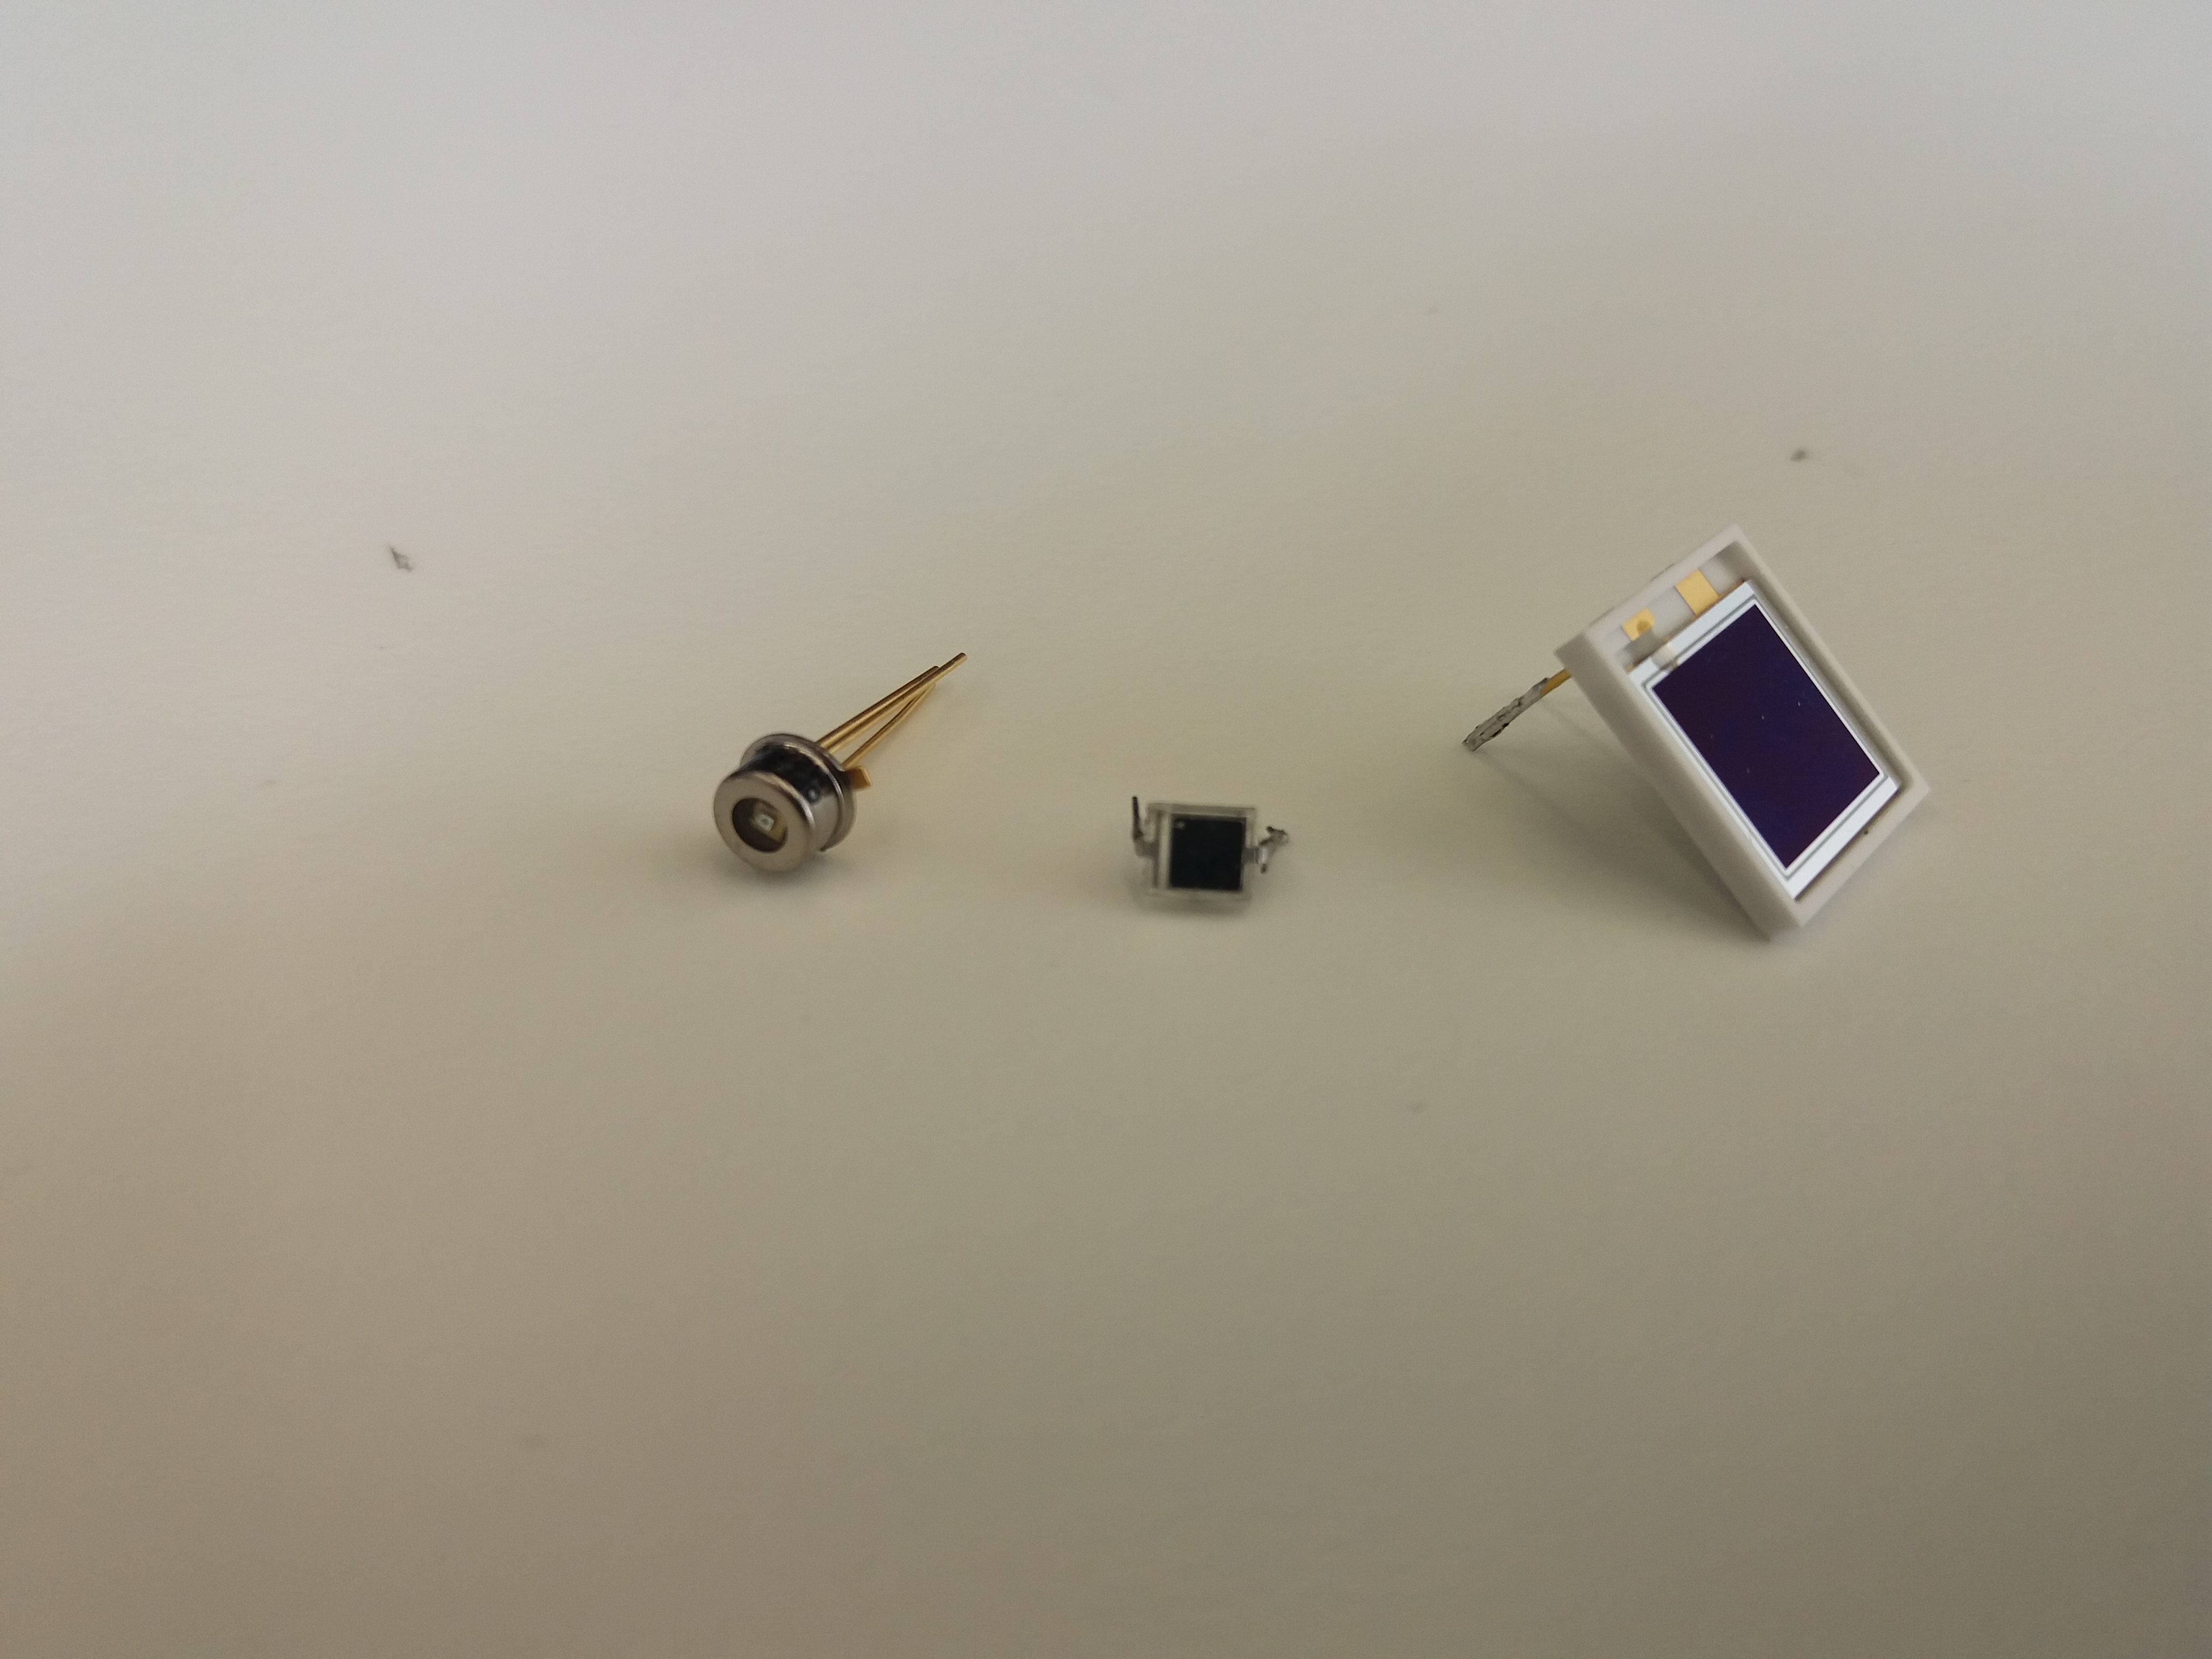
\includegraphics[scale=0.1, angle = 0]{./pictures/PINdiodes.png}
 \caption{PIN diodes - OPF430, BPW34 and S14605.}
 \label{PIN diodes}

\end{figure}

\subsection{Hamamatsu S14605}
The professional S14605 is designed for use as a direct radiation detector. It has a very large light sensitive area and low capacitance.
%The professional S14605 is designed to be used as a direct radiation detector. It offers a very large photosensitive area and a low capacitance.

Parameters \cite{datS14605}:
\begin{itemize}
\item Maximum reverse voltage $U_\textrm{R}$: 150 V
\item Photosensitive area: 81 mm$^2$
\item Capacitance: 25 pF at $U_\textrm{R} = 100$ V
\item Dark current: 8 nA at $U_\textrm{R} = 100$ V
\item Depletion layer: 0.5 mm
\item Cost: 5000 CZK
\end{itemize}

%\begin{figure}[H]
% \centering
% 
\includegraphics[scale=0.35, angle = 0]{./pictures/NoPicture.jpg}
% \caption{Hamamatsu S14605.}
% \label{S14605}
% 
%\end{figure}



\subsection{BPW34}
BPW34 is a very inexpensive radiation detector. There was a manual \cite{betaBPW} on how to use BPW34 as a beta particle detector, and since it is a Si PIN diode, it is worth a try and test for our gamma detection purposes.
%BPW34 is a very low cost radiation detector. There was manual \cite{betaBPW} how to use BPW34 as a beta particle detector, and since it is a Si PIN diode, it worths a try and test it for our gamma detection purposes.



Parameters \cite{datBPW34}:
\begin{itemize}
\item Maximum reverse voltage $U_\textrm{R}$: 32 V
\item Photosensitive area: 7.5 mm$^2$
\item Capacitance: 25 pF at $U_\textrm{R} = 3$ V
\item Dark current: 2 nA at $U_\textrm{R} = 10$ V
\item Depletion layer: not specified
\item Cost: 11 CZK
\end{itemize}

%\begin{figure}[H]
% \centering
% 
\includegraphics[scale=0.35, angle = 0]{./pictures/NoPicture.jpg}
% \caption{BPW34.}
% \label{BPW34}
% 
%\end{figure}
\subsection{OPF430}
OPF430 was originally intended as a low cost detector for fibre optic applications. However, there was a publication \cite{RAMIREZJIMENEZ2003577} which described the possibility of using similar diode OPF420 in low energy gamma spectroscopy chains as a low cost detector.
%OPF430 is originally ment to be a low-cost detector for fiber optic applications. However, there was publication \cite{RAMIREZJIMENEZ2003577}, which described the possibility of using similar diode OPF420 in low-energy gamma spectroscopy chains as a low-cost detector.

Parameters \cite{datOPF430}:
\begin{itemize}
\item Maximum reverse voltage $U_\textrm{R}$: 100 V
\item Photosensitive area: not specified, smaller than BPW34
\item Capacitance: 1.5  pF at $U_\textrm{R} = 5$ V
\item Dark current: 0.1 nA at $U_\textrm{R} = 5$ V
\item Depletion layer: not specified
\item Cost: 340 CZK
\end{itemize}

%\begin{figure}[H]
% \centering
% 
\includegraphics[scale=0.35, angle = 0]{./pictures/NoPicture.jpg}
% \caption{OPF430.}
% \label{OPF430}
% 
%\end{figure}
% %%%%%%%%%%%%%%%%%%%%%%%% End of file %%%%%%%%%%%%%%%%%%%%%%%%
